\chapter{Binárne vyhľadávanie a logaritmy}
\label{sect:binarysearch}

Hrajme takúto hru: myslím si číslo od 1 po $N$ a tvojou úlohou je ho uhádnuť. Môžeš
sa opýtať na nejaké číslo a ja ti odpoviem \cmd{viac}, \cmd{menej} alebo \cmd{uhádol si}.
Ako budeš hádať, aby si čo najskôr uhádol? Koľko otázok na to budeš potrebovať?

 
Povedzme, že $N=1000$. Ak sa na začiatku opýtaš na $5$ a máš šťastie, dostaneš odpoveď
\cmd{menej} a vieš, že to môže byť iba 1, 2, 3, alebo 4. Ale ak šťastie nemáš,
príliš si si nepomohol: môže to byť čokoľvek medzi 6 a 1000. Ale možnože nehrám férovo a
podvádzam: v skutočnosti si nemyslím číslo, ale čakám, čo sa ma opýtaš. Ak sa spýtaš na $5$,
odpoviem ti \cmd{viac} a budem sa tváriť, že som si myslel číslo medzi 6 a 1000 (potom 
to už musím dodržať, lebo inak by si zistil, že som podvádzal). Najlepšie, čo môžeš 
v tejto situácii urobiť,
je opýtať sa na číslo v strede. Koľko otázok potrebuješ, aby si touto stratégiou 
uhádol číslo? Jednoduchšie je pýtať sa opačnú otázku: pre aký najväčší rozsah $N$
ti stačí $n$ otázok? Poďme postupne. Ak môžeš položiť 1 otázku, tak $N$ môže byť najviac 
$3$: ak si myslím číslo od 1 po 3, tak sa najprv spýtaš na 2, a keď si neuhádol a dostal
si odpoveď \cmd{menej}, vieš, že som si myslel 1, a ak si dostal odpoveď \cmd{viac} tak vieš,
že som si myslel 3. Keď si ale myslím číslo od 1 po 4, jedna otázka ti nestačí: spýtaš sa
na 2, je odpoviem \cmd{viac} a teraz nevieš, či som si myslel tri alebo štyri.


Čo ak máš dve otázky? Ak si myslím číslo od 1 po 7, vieš ho zistiť: opýtaš sa na 4. Ak ti
poviem \cmd{menej} máš jednu otázku na to, aby si uhádol číslo od 1 do 3 (tri čísla jednou
otázkou, to vieš), ak ti
odpoviem \cmd{viac} máš jednu otázku na to, aby si uhádol číslo od 5 do 7 (zase tri čísla
jednou otázkou). Ak máš tri otázky, môžem si myslieť číslo od 1 po 15: prvou otázkou
za opýtaš na 8 a ostanú ti dve otázky na uhádnutie čísla spomedzi siedmich.


Keď si označím $m_n$ najväčšie číslo, ktoré vieš $n$ otázkami uhádnuť, tak sme videli,
že $m_1=3$, $m_2=7$, $m_3=15$. Vždy, keď máš o jednu otázku viac, vieš robiť to isté,
preto $m_{n+1}=2m_n+1$ (ak máš $n+1$ otázok, opýtaš sa na to 1 číslo v strede a 
v každom prípade ti ostane $n$ otázok na uhádnutie čísla z rozsahu  $m_n$). Ľahko si overíme,
že $m_n=2^{n+1}-1$. Pre malé hodnoty to vieme priamo:
\begin{align*}
  m_1&=2^2-1=4-1=3 \\
  m_2&=2^3-1=8-1=7 \\
  m_3&=2^4-1=16-1=15
\end{align*}

potom ak už vieme, že $m_n=2^{n+1}-1$, tak vieme aj, že $m_{n+1}=2m_n+1=2(2^{n+1}-1)+1=
2\cdot2^{n+1}-2+1=2^{n+2}-1$. Z toho potom vieme dokázať, že $m_{n+2}=2^{n+3}-1$ a tak ďalej.
Teda $2^{n+1}$ je prvé číslo, na ktoré potrebuješ viac ako $n$ pokusov. 


Naspäť k prvej otázke: ak hádam čísla z rozsahu 1 až $N$, koľko otázok potrebuješ? Nech
je to číslo $n$, potom $2^{n+1}-1\ge N$, t.j. $2^n\ge(N+1)/2$. Takéto číslo má svoje meno:\indexItem{Mat}{logaritmus}
volá sa {\em logaritmus}. Presne povedané: \cmd{logaritmus z čísla $n$ je také číslo $x$,
že $2^x=n$}. V našom prípade umocňujeme dvojku, preto hovoríme, že používame 
{\em logaritmus pri základe 2}. Napr. $\log16=4$, lebo $2^4=2\cdot2\cdot2\cdot2=16$. 
Umocňovanie aj logaritmy sa dajú prirodzene rozšíriť aj na desatinné čísla\phantomsection\label{page:umocnovanie}\footnote{%
  Ak $b$ je celé číslo, umocňovanie je jednoduché: \indexItem{Mat}{umocnenie na neceločíselný exponent}
  $a^b=\overbrace{a\cdot a\cdots a}^b$. Preto platí 
  $a^{b+c}=\overbrace{a\cdots a}^b\cdot\overbrace{a\cdots a}^c=a^b\cdot a^c$.
  Podobne $a^{bc}=
  \overbrace{a\cdots a}^b\cdot
  \overbrace{a\cdots a}^b
  \cdots\overbrace{a\cdots a}^b=(a^b)^c$. Ak chceme,
  aby tieto pravidlá stále platili, koľko by bolo $a^{-1}$? Musí platiť
  $a^{-1}\cdot a^1=a^{-1+1}=a^0=1$. Preto $a^{-1}=\frac{1}{a}$.
  Koľko by bolo $a^\frac{1}{2}$? Musí platiť
  $a=a^1=a^{\frac{1}{2}+\frac{1}{2}}=a^\frac{1}{2}\cdot a^\frac{1}{2}$. Preto 
  $a^\frac{1}{2}=\sqrt{a}$. Podobne $a^\frac{1}{p}$ je také číslo $x$, že $x^p=a$.
  Také číslo voláme $p$-ta odmocnina z $x$ a značíme $\sqrt[p]{x}$.
  Teraz vieme, že $a^\frac{p}{q}=a^{\frac{1}{q}p}=(\sqrt[q]{a})^p$ a 
  $a^{-\frac{p}{q}}=a^{\frac{p}{q}\cdot(-1)}=((\sqrt[q]{a})^p)^{-1}=\frac{1}{(\sqrt[q]{a})^p}$.

  Ak povieme, že $\log a$ je také číslo $b$, že $2^b=a$, máme logaritmus pre všetky čísla,
  nielen pre mocniny dvojky. Z pravidiel pre umocňovanie vyplýva, že 
  $\log(ab)=\log a+\log b$, pretože $\log(ab)$ je také číslo, že $2^{\log(ab)}=ab$.
  Lenže $a=2^{\log a}$ a $b=2^{\log b}$, preto $ab=2^{\log a}2^{\log b}=2^{\log a+\log b}$,
  takže $2^{\log(ab)}=2^{\log a+\log b}$ a preto aj $\log(ab)=\log a+\log b$.
  Rovnako vieš zdôvodniť, že $\log(a/b)=\log a-\log b$, $\log(a^b)=b\log a$ a pod.
}, preto si môžeme nakresliť graf funkcie $\log(x)$:


\begin{tikzpicture}
\begin{axis}[
  %title={},
  width=\textwidth, 
  height=7cm,
  xlabel=$x$,
  ylabel=$ $,
  scaled x ticks=false,
  scaled y ticks=false,
  domain=0:2000,
  samples=200,
  xmin=0,
  xmax=2000,
  /pgf/number format/.cd,
        1000 sep={}
]
  \addplot[no markers,red!50!white]{log2(x)};
\end{axis}
\end{tikzpicture}

Všimni si, že stále rastie, ale čím ďalej, tým pomalšie.
Napr. $\log(4398046511104)$ je $42$.


Zoberme si teraz programátorskú úlohu, ktorá sa podobá našej hre. Predpokladajme,
že máme pole \prg!int a[n];! v ktorom sú rôzne čísla utriedené on najmenšieho po najväčšie.
Našou úlohou je napísať funkciu,
ktorá pre nejaké zadané číslo \vb{x} zistí, či sa v poli \vb{a} nachádza alebo nie.
Môžme to spraviť priamočiaro:

\vskip 2ex
\vbox{
\begin{lstlisting}[] 
bool find(int n, int *a, int x) {
  for (int i = 0; i < n; i++)
    if (a[i] == x) return true;
  return false;
}
\end{lstlisting}
}

Táto funkcia má evidentne lineárnu zložitosť. Vieme to spraviť lepšie? Môžeme zvoliť
rovnakú stratégiu ako pri hádacej hre: pozrieme sa do stredu poľa, zistíme, či je
tam väčšie alebo menšie číslo a podľa toho hľadáme buď v ľavej alebo v pravej časti.
Budeme mať teda cyklus, v ktorom budeme kontrolovať menšie a menšie intervaly.
Okraje intervalu si budeme pamätať v premenných \vb{l} a \vb{r}. Stred intervalu
\vb{m} vyrátame ako priemer \vb{l} a \vb{r}, t.j \vb{m=(l+r)/2}. Treba si dať trochu
pozor na to, kedy skončiť, ale celá
funkcia môže vyzerať nejak takto: \indexItem{Alg}{binárne vyhľadávanie}

\vskip 2ex
\vbox{
\begin{lstlisting}[] 
bool najdi(int n, int *a, int x) {
  int l = 0, r = n - 1, m;
  if (a[l] > x || a[r] < x) return false;
  if (a[l] == x || a[r] == x) return true;
  while (l < r - 1) {
    m = (l + r) / 2;
    if (a[m] == x) return true;
    if (a[m] > x)
      r = m;
    else
      l = m;
  }
  return false;
}
\end{lstlisting}
}

Prečo to funguje? Na začiatku skontrolujeme okrajové podmienky.
Počas celého cyklu potom vieme, že hľadané číslo je určite ostro väčšie \vb{a[l]} a zároveň ostro menšie ako \vb{a[r]},\footnote{všimni si, 
že na začiatku cyklu to platí a v cykle vždy meníme \vb{l} a \vb{r} tak, aby to ostalo zachované}
preto keď \vb{l} a \vb{r} sú susedné, vieme že hľadané číslo sa v poli nenachádza. 
Predpokladajme, že v nasledovnom poli
hľadáme číslo $42$. Výpočet by potom mohol vyzerať takto:



\centerline{
\begin{tikzpicture}[scale=0.5]
  \def\pal#1{\ifnumequal{#1}1{yellow!20!white}{\ifnumequal{#1}2{green!20!white}{red!10!white}}}
  \def\krb(#1)#2#3{
    \filldraw[fill=\pal#2](#1,0) rectangle node[align=center]{\vb{#3}} (#1+1,1);
    \pgfmathtruncatemacro{\tmp}{#1-1}
    \node[anchor=north] at(#1+0.5,-0.1){{\small\roboto \tmp}};
  }
  \def\mark(#1)#2{
    \draw[blue, ->, shorten <= 2, shorten >=2] 
    (#1+0.5,1.8) node[anchor=south]{{\small\roboto #2}}  -- (#1+0.5,1);
  }
  \def\strip(#1,#2){
    \pgfmathtruncatemacro{\tmp}{(#1+#2)/2}
    \foreach \v [count=\i] in {12,13,15,26,27,28,30,33,35,40,42,47,63,64,67,80} {
      \def\clr{2}
      \ifnumless{\i}{#1}{\def\clr{3}}{}
      \ifnumgreater{\i}{#2}{\def\clr{3}}{}
      \ifnumequal{\i}{#1}{\def\clr{1}}{}
      \ifnumequal{\i}{#2}{\def\clr{1}}{}
      \ifnumequal{\i}{\tmp}{\def\clr{1}}{}
      \krb(\i){\clr}{\v}
    }
    \mark(#1){l}
    \mark(#2){r}
    \mark(\tmp){m}
  }

  \foreach \l/\r [count=\i] in {1/16,8/16,8/12,10/12} {
    \begin{scope}[shift={(0,-4*\i)}]
      \strip(\l,\r)
    \end{scope}
  }
\end{tikzpicture}}

 Funkcia \vb{najdi} má logaritmickú zložitosť. 
Môžeš sa pýtať, načo je logaritmická zložitosť
dobrá, keď už na samotné prečítanie vstupného poľa potrebujeme lineárnu zložitosť. 
Častokrát potrebuješ počas tvojho programu veľakrát riešiť podobný problém. Napríklad
keď hľadáš cestu v bludisku, na každej križovatke sa musíš rozhodnúť, kam odbočiť. Vtedy
má zmysel, aby rozhodovacia funkcia mala zložitosť menšiu ako lineárnu, lebo 
vstup je už raz načítaný v pamäti. Iné použitie binárneho vyhľadávania, ktoré uvidíš,
je podobné ako v hre na začiatku kapitoly: v pamäti nie je uložené celé pole, ale 
máš len funkciu, ktorá ti hovorí \cmd{viac} alebo \cmd{menej}.

 Malá odbočka: ak máš zložitejší cyklus, ako napríklad v tomto prípade a chceš \indexItem{Alg}{invariant}
sa uistiť, že program funguje správne, je dobré vymyslieť si tzv. {\em invariant}.
Invariant je podmienka, ktorá platí vždy na začiatku cyklu. V tomto prípade 
invariant hovorí, že ak je hľadané číslo v poli, je napravo od \vb{l} a naľavo od \vb{r}.
Ak invariant platí na začiatku jednej iterácie cyklu, určite platí aj na začiatku ďalšej:
ak sa začala ďalšia iterácia, tak hľadané číslo nie je \prg!a[m]! a určite 
sa nachádza medzi novým \vb{l} a novým \vb{r}. Zároveň vidno, že vzdialenosť \vb{l}
a \vb{r} sa v každej iterácii cyklu zhruba spoloviční. Takto by sa dalo dokázať,
že program vždy skončí po logaritmickom počte iterácií a dá správnu odpoveď.
Podobný spôsob rozmýšľania sme použili pri algoritme {\em Insertion Sort} v 
kapitole~\ref{sect:zlozitost} aj pri úlohe o klaunoch v kapitole~\ref{sect:stack}.

\begin{uloha}
  V pamäti je pole \prg!a!, ktoré obsahuje $n$ prirodzených čísel
  utriedených od najmenšieho. Napíš funkciu, ktorá dostane ako parameter 
  číslo $k$ a povie, koľkokrát sa $k$ nachádza v poli. Funkcia by mala
  mať logaritmickú zložitosť.
\end{uloha}

\begin{uloha}
  V pamäti sú dve usporiadané polia \vb{a} a \vb{b}, pričom každé obsahuje $n$ čísel.
  Napíš funkciu, ktorá zistí, ktorý prvok by bol na $n$-tej pozícii, keby sa obe
  polia spoločne utriedili. Napr. pre $n=6$ a polia \vb{3 6 9 12 15 18} a 
  \vb{2 4 6 8 10 12} je výsledok $8$, lebo spoločné utriedené pole
  je \vb{2 3 4 6 6 8 9 10 12 12 15 18} a v ňom na šiestom mieste je osmička.
  Funkcia by mala mať logaritmickú zložitosť.
\end{uloha}

Častokrát je pri riešení úloh užitočný prístup 
''{\em binárne vyhľadávanie nad výsledkami}''. V ňom, podobne ako v hre s hádaním čísla, nemáme
pole, ale iba nejakú funkciu, ktorej sa viem opýtať. 
Ukážem ti to na príklade. 
Začnime s úplne nesúvisiacou úlohou:

\begin{uloha}
  \label{uloha:nulyfaktorialu}
  Na vstupe je číslo $n$. Napíš program, ktorý zistí, koľko núl je na konci čísla
  $n!$ ($n!$ znamená faktoriáal ako v úlohe~\ref{uloha:faktorial}). 
  Napr. pre vstup $6$ je výstup $1$, pre vstup $11$ je výstup $2$ (lebo
  $11!=39916800$), pre $123$ je výstup $28$.
\end{uloha}

S touto úlohou je ten problém, že $n!$ veľmi rýchlo rastie a veľmi skoro sa nezmestí ani
do premennej typu \prg!unsigned long long int!. Môžeš zobrať riešenie 
úlohy~\ref{uloha:faktorial} a jednoducho počet núl na konci zrátať, ale
dá sa to urobiť lepšie. 
Každé prirodzené číslo $n$ sa dá rozložiť na súčin prvočísel\footnote{o prvočíslach bola\indexItem{Mat}{provčíselný rozklad} 
úloha~\ref{uloha:primetest}} takto: začnem s číslom $n$; ak je prvočíslo, tak super,
inak má deliteľa a platí $n=a\cdot b$. No a v rozklade pokračujem pre $a$ aj $b$ dokola,
až sa dopracujem k prvočíslam. Napríklad $120=20\cdot6=4\cdot5\cdot2\cdot3=
2\cdot2\cdot5\cdot2\cdot3$. Je užitočné si uvedomiť, že síce môžem pri rozklade postupovať
rôzne, vždy sa dostanem k rovnakým prvočíslam (možno
v inom poradí)\footnote{%
  Prečo to platí? Euklides by uvažoval takto: zoberiem si najmenšie číslo $s$,
  pre ktoré môžem mať dva rôzne rozklady, t.j. 
  $s=p_1\cdotp_2\cdots p_m=q_1\cdot q_2\cdots q_n$, kde $p$-čka aj $q$-čka sú prvočísla.
  Keby nejaké $p_i=q_j$, tak ním $s$ vydelím a dostanem menšie číslo s dvoma rôznymi
  rozkladmi, takže $p$-čka a $q$-čka sú rôzne. Dajme tomu, že $p_1<q_1$ (keby to tak nebolo,
  tak premenujem $p$-čka a $q$-čka). Ak si označím $P=p_2\cdot p_3\cdots p_m$
  a $Q=q_2\cdot q_3\cdots q_n$, tak vidím, že
  $$s=p_1\cdot P = q_1\cdot Q$$
  Z obidvoch strán môžem odrátať $p_1Q$ a stále dostanem nezáporné číslo, lebo $p_1<q_1$.
  Budem teda mať
  $$p_1P-p_1Q=q_1Q-p_1Q$$
  Teraz využijem, že $ab-ac=a(b-c)$, čo ľahko vidno z plochy obdĺžnikov

  \centerline{\tikz[xscale=0.45,yscale=0.6]{
    \def\lup(#1,#2)#3{\draw decorate[
       decoration={brace, amplitude=2ex}]{
       (#1,1) -- (#2,1) node [align=center,midway,anchor=south,yshift=2ex] {#3}
        };
        }

    \filldraw[fill=green!10!white](0,0) rectangle (3,1);
    \filldraw[fill=yellow!10!white](3,0) rectangle (5,1);
    \lup(0,3){$b-c$}
    \lup(3,5){$c$}
    \node[rotate=90,anchor=south] at(0,0.5){$a$};
    \draw decorate[
       decoration={brace, amplitude=2ex}]{
       (5,0) -- (0,0) node [align=center,midway,anchor=north, inner sep=3ex] {$b$}
        };
    
      }}
  a dostanem
  $$p_1(P-Q)=(q_1-p_1)Q<s$$
  Číslo $(q_1-p_1)Q$ má jednoznačný rozklad na prvočísla (lebo je menšie ako $s$), a keďže
  $p_1$ je prvočíslo, ktoré ho delí, 
  tak niekde v tom rozklade je. Ale nemôže byť v rozklade $Q$, lebo
  ten sa skladá so samých $q$-čok a vieme, že $p$-čka a $q$-čka sú rôzne. Preto $p_1$ sa
  nachádza v rozklade $q_1-p_1$. Lenže ak $p_1$ delí $q_1-p_1$, tak určite delí aj
  $q_1$. Ale to nemôže, lebo $q_1$ je iné prvočíslo. To celé znamená, že nemôže existovať
  najmenšie (a teda žiadne) číslo $s$, ktoré by nemalo jednoznačný rozklad na prvočísla.
}. Napr. $120=5\cdot24=5\cdot6\cdot4=5\cdot2\cdot3\cdot2\cdot2$.

Každá nula na konci čísla znamená, že číslo sa dá vydeliť desiatimi, a teda v prvočíselnom
rozklade je jedna päťka a jedna dvojka. Napríklad 
$$11! = 11\cdot10\cdot9\cdot8\cdot7\cdot6\cdot5\cdot4\cdot3\cdot2$$
čo keď rozpíšeme, budeme mať
$$11! = 11\cdot7\cdot5^2\cdot3^4\cdot2^8$$
Na konci teda budú dve nuly. V prvočíselnom rozklade $n!$ bude vždy viac dvojek ako pätiek,
preto stačí rátať päťky. Napr. pre $26!$ ich narátaš $6$: po jednej v číslach $5$, $10$, $15$,
$20$ a dve v čísle $25$. Teraz sa už úloha~\ref{uloha:nulyfaktorialu} dá vyriešiť ľahko, napr.


\begin{lstlisting}[] 
int nuly(int n) {
  int z = 0;
  while (n > 1) {                        // pre každé číslo
    for (int i = 5; i <= n; i = i * 5)   // všetky mocniny 5
      if (n % i == 0) z++;               // ktoré ho delia
    n--;
  }
  return z;
}
\end{lstlisting}


Ako to ale súvisí s našim rozprávaním o binárnom vyhľadávaní? Pozrime sa na ''opačnú''
úlohu:

\begin{uloha}
  Na vstupe je číslo $x>0$. Napíš program, ktorý vypíše najmenšie $n$ také, že na konci
  $n!$ je $x$ núl.
\end{uloha}

Mohol by som ísť v cykle postupne od 1, vždy zavolať funkciu \vb{nuly} a zastaviť sa
pri prvom čísle, ktoré má aspoň $x$ núl. 

 
Čísla, ktorých faktoriál
má na konci aspoň $x$ núl budem volať {\em dobré}, ostatné sú {\em zlé}.
Pretože \hbox{$(n+1)!=(n+1)\cdot n!$,} tak všetky delitele $n!$ sú aj delitele $(n+1)!$. To znamená,
že pre rastúce $n$, núl na konci $n!$ iba pribúda, nikdy neubúda. Preto v postupnosti
$1,2,3,4,\ldots$ sú najprv zlé čísla a potom od istého čísla už sú všetky dobré.
Keďže $x>0$, viem, že $1$ je určite zlé číslo.
Keby som vedel aspoň jedno dobré číslo $n_0$, môžem použiť binárne vyhľadávanie:
pozriem sa, či je $n_0/2$ dobré. Ak áno, najmenšie dobré číslo bude medzi $1$ a $n_0/2$,
ak nie, bude medzi $n_0/2$ a $n_0$. Potom budem pokračovať rovnako ako pri binárnom
vyhľadávaní: vždy bude platiť, že \vb{l} je zlé a \vb{r} dobré číslo. Keď nakoniec
budú \vb{l} a \vb{r} susedné, zjavne \vb{r} je najmenšie dobré číslo.
Ako ale nájdem $n_0$? Začnem od jednotky a budem vždy skúšať dvojnásobok:
$2,4,8,16,\ldots,2^i,\ldots$. Časom sa dostanem až k nejakému dobrému číslu $n_0=2^i$, 
ktoré určite
nebude väčšie ako dvojnásobok najmenšieho dobrého čísla (lebo $n_0/2$ ešte dobré nebolo).
Dostanem sa k nemu na $i$ pokusov. Keďže $i$ je také číslo, že $2^i=n_0$, platí
$i=\log(n_0)$. Binárne vyhľadávanie tiež urobí najviac $\log(n_0)$ pokusov, dokopy
teda môj program zavolá funkciu \vb{nuly} najviac $2\log(n)+3$ krát (čiže počet
pokusov je logaritmický). 
Program by mohol vyzerať takto:


\begin{lstlisting}[] 
int main() {
  int x;
  cin >> x;
  int l = 1, r = 1, m;
  while (nuly(r) < x) r = 2 * r;
  while (l < r - 1) {
    m = (l + r) / 2;
    if (nuly(m) < x) l = m;
    else r = m;
  }
  cout << r << endl;
}
\end{lstlisting}

Pre $x=5$ by sa postupne skúšali tieto hodnoty (červené sú zlé čísla a zelené dobré,
modré štvorčeky sú tie, na ktoré sa volá funkcia \vb{nuly}):


  \def\pal#1{\ifnumequal{#1}1{yellow!20!white}{\ifnumequal{#1}2{green!20!white}{red!10!white}}}
  \def\krb(#1)#2{
    \filldraw[fill=\pal#2](#1,0) rectangle (#1+1,1);
    \node[anchor=north] at(#1+0.5,-0.1){{\scriptsize\roboto #1}};
  }
  \def\mark(#1)#2#3{
    \if1#3\draw[blue,thick](#1,0)rectangle(#1+1,1);\fi
    \draw[blue, ->, shorten <= 2, shorten >=2] 
    (#1+0.5,1.8) node[anchor=south]{{\small\roboto #2}}  -- (#1+0.5,1);
  }
  \def\strip{
    \foreach \i in {1,...,34} {
      \def\clr{2}
      \ifnumless{\i}{25}{\def\clr{3}}{}
      \krb(\i){\clr}
    }
  }

\centerline{
\begin{tikzpicture}[scale=0.4]
 \strip
  \foreach \i in {1,2,4,8,16} {
    \draw[blue] (\i+0.5,1) to [out=45,in=135]  (2*\i+0.5,1);
     \draw[blue,thick](\i,0)rectangle(\i+1,1);
  }
     \draw[blue,thick](32,0)rectangle(32+1,1);

  \foreach \l/\r [count=\i] in {1/32,16/32, 24/32} {
    \begin{scope}[shift={(0,-4*\i)}]
      \pgfmathtruncatemacro{\tmp}{(\l+\r)/2}
      \strip
      \mark(\l){l}0
      \mark(\r){r}0
      \mark(\tmp){m}1
    \end{scope}
  }
\end{tikzpicture}}

\centerline{
\begin{tikzpicture}[scale=0.4]
  \foreach \l/\r [count=\i] in {24/28,24/26} {
    \begin{scope}[shift={(0,-4*\i)}]
      \pgfmathtruncatemacro{\tmp}{(\l+\r)/2}
      \strip
      \mark(\l){l}0
      \mark(\r){r}0
      \mark(\tmp){m}1
    \end{scope}
  }
    \begin{scope}[shift={(0,-4*3)}]
      \def\l{24}
      \def\r{25}
      \pgfmathtruncatemacro{\tmp}{(\l+\r)/2}
      \strip
      \mark(\l){l}0
      \mark(\r){r}1
    \end{scope}
\end{tikzpicture}}




 Aký je rozdiel v rýchlosti medzi týmto programom a pôvodnou verziou, ktorá
volala funkciu \vb{nuly} zaradom? Pre $n=20000$ mi pôvodná verzia bežala minútu
a 17 sekúnd, kým tento program zbehol za 48 ms. 


Skúsme spoločne spraviť ešte jeden príklad:

\begin{uloha}
  Máme \vb{n} displejov, ktoré ukazujú hodnoty 
  \hbox{\vb{p[0]}, \vb{p[1]}, \ldots, \vb{p[n-1]}.}
  Pre $i$-ty displej môžeme zaplatiť  \vb{m[i]} peňazí, aby sa
  hodnota na ňom zvýšila o $1$.
  Máme k dispozícii \vb{b} peňazí. Našim cieľom je, aby  displeje
  ukazovali čo najväčšie čísla, teda aby najmenšie číslo, ktoré ukazuje nejaký
  displej, bolo čo najväčšie. Napíš program, ktorý pre zadané polia \vb{p} a
  \vb{m} a rozpočet \vb{b} zistí, aké najväčšie čísla môžu displeje ukazovať.
  Napr. ak \vb{p} je \hbox{\vb{[1 2 3]}}, \vb{m} je \hbox{\vb{[2 3 1]}} a \vb{b} je $7$, tak
  výsledok je $3$: dvakrát zaplatíme po $2$, aby sa prvý displej dostal na $3$
  a raz zaplatíme $3$, aby sa aj druhý displej dostal na $3$. Spotrebovali sme akurát $7$
  peňazí a dosiahli sme, že na všetkých displejoch je aspoň trojka.
\end{uloha}

Opäť použijeme binárne vyhľadávanie nad výsledkami. Máme nájsť maximálne číslo, ktoré
vieme s našim rozpočtom \vb{b} dosiahnuť. Ako by sa dalo zistiť, či vieme dosiahnuť
nejaké číslo \vb{k}? To je jednoduché: ak je na nejakom displeji číslo \vb{p[i]} menšie
ako \vb{k}, musíme doplatiť \vb{m[i]*(k-p[i])}, aby sme ho dostali na hodnotu \vb{k}.
Toto skontrolujeme pre všetky displeje a overíme, či nám na to vystačia peniaze:

\begin{lstlisting}
bool test(int k) {
  int sum = 0;
  for (int i = 0; i < n; i++)
    if (p[i] < k) sum += m[i] * (k - p[i]);
  return sum <= b;
}
\end{lstlisting}

V hlavnom programe použijeme binárne vyhľadávanie. Budeme udržiavať invariant, že
\vb{l} vždy dosiahnuť vieme a \vb{r} nevieme. Cyklus skončí, ak budú \vb{l}
a \vb{r} susedné, takže \vb{l} musí byť najväčšie číslo, ktoré sa dá dosiahnuť.

\begin{lstlisting}
 while (l < r - 1) { 
    x = (l + r) / 2;
    if (test(x))
      l = x;
    else
      r = x;
  } 
  cout << l << endl;
\end{lstlisting}


Posledná otázka je, ako na začiatku nastaviť \vb{l} a \vb{r}. Aj keby sme nezaplatili nič,
vieme získať hodnotu najmenšieho displeja, preto začneme s \prg!l=min(p)!, kde funkcia
\vb{min} vyráta najmenšiu hodnotu z poľa. 

\begin{lstlisting}
int min(vector<int> &a) {
  int res = a[0];
  for (int i = 1; i < a.size(); i++)
    if (a[i] < res) res = a[i];
  return res;
} 
\end{lstlisting}

Ak by bol najväčší displej najlacnejší možný (t.j. stačilo by zaplatiť 1 na jeho zväčšenie) a všetky peniaze by
sme investovali doňho, aj tak nedosiahneme \prg!r=max(p) + b + 1!.

 Tu je niekoľko úloh podobného typu:

\begin{uloha}
  Máme $n$ obdĺžnikov s výškami \vb{a[0]},\ldots,\vb{a[n-1]}, ktoré môžeme {\em odpíliť}
  takto: nastavíme výšku \vb{h} a z každého obdĺžnika zoberieme časť, ktorá prečnieva
  cez \vb{h}. Napíš program, ktorý pre zadané pole \vb{a} a číslo \vb{m} nájde
  najväčšie číslo \vb{h}, pri ktorom z odpílených obdĺžnikov  zozbierame aspoň \vb{m}.
  Napr. pre obdĺžniky \vb{14 42 40 26 46} a \vb{m}$=20$ je odpoveď $36$, lebo s
  výškou \vb{h}$=36$ pozbierame
$0+6+4+0+10=20\ge20$.


  \centerline{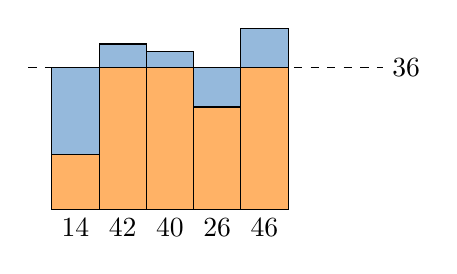
\begin{tikzpicture}[xscale=0.6,yscale=0.05]
  \def\bar(#1,#2){
    \node[anchor=north] at (#1+0.5,0) {$#2$};
    \ifnumless{#2}{36}{
    \filldraw[draw=black,fill=\prf](#1,0) rectangle (#1+1,#2);
  }{
    \filldraw[draw=black,fill=\prf](#1,0) rectangle (#1+1,36);
    \filldraw[draw=black,fill=\act](#1,36) rectangle (#1+1,#2);
  }
  }
  \def\prf{orange!60!white}
  \def\rst{rgb:green,5;yellow,4;blue,2;black,3}
  \def\act{rgb:blue,8;green,4;white,17}

    \foreach \x[count=\i] in {14,42,40,26,46} {
      \bar(\i,\x)
    }
    \draw[dashed](0.5,36)--(8,36) node[anchor=west]{$36$};
  \end{tikzpicture}}

\end{uloha}


\begin{uloha}
  Na rovnej čiare je \vb{n} bodov v pozíciách $\vb{a[0]} \ldots \vb{a[n-1]}$.
  Okrem toho je zadané číslo \vb{c}$>1$. Treba vybrať \vb{c} bodov tak,
  aby boli od seba čo najďalej (t.j. aby minimálna vzdialenosť medzi 
  dvoma susednými vybratými bodmi bola čo najmenšia). Napíš program, 
  ktorý vypočíta túto vzdialenosť.
  Napr. pre vstup
  \vb{1 2 8 4 9} a \vb{c}$=3$ je odpoveď \vb{3},
  lebo keď vyberieme body $1,4,8$, najbližšie dva sú $1$ a $4$ vo vzdialenosti $3$.

  
  \centerline{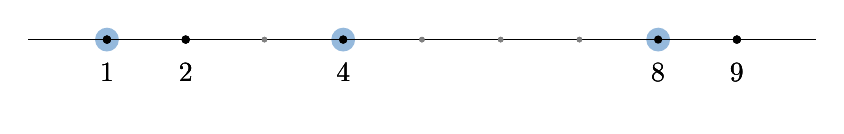
\begin{tikzpicture}
    \foreach \x in {1,4,8} {
      \fill[fill={rgb:blue,8;green,4;white,17}] (\x,0) circle (1ex);
      \draw(0,0) -- (10,0);
      \foreach \x in {1,...,9}{
        \fill[gray](\x,0) circle (1pt);
      }
      \foreach \x in {1,2,4,8,9}{
        \fill(\x,0) circle (1.5pt) node[anchor=north, inner sep=2ex]{$\x$};
      }
    }
  \end{tikzpicture}}
\end{uloha}

\begin{uloha}
  \def\tmpA{\textcolor{red}{{\bfseries A}}}
  \def\tmpB{\textcolor{blue}{{\bfseries B}}}
  \def\tmpC{\textcolor{green!50!black}{{\bfseries C}}}
  K dispozícii máme $k$ sád kartičiek s rôznymi znakmi, pričom z \vb{i}-tej
  sady máme k dispozícii \vb{a[i]} kartičiek. Všetkých kartičiek dokopy je \vb{n}.
  Napíš program, ktorý zistí, koľko najviac rovnakých riadkov z kartičiek vieme poskladať.
  Napr. pre $k=3$, $n=4$ a vstup \vb{7 6 3} je správna odpoveď \vb{3}: máme
  7 kartičiek \tmpA, 6 kartičiek \tmpB~a 3 kartičky \tmpC, preto môžeme spraviť
  tri riadky \tmpA\tmpA\tmpB\tmpC~ (a ostanú nám kartičky \tmpA\tmpB\tmpB\tmpB), 
  ale
  nemôžeme spraviť 4 riadky.
\end{uloha}

\begin{uloha}
  Máme \vb{n} displejov, ktoré majú na začiatku hodnoty \vb{a[0]},\ldots,\vb{a[n-1]}
  a každý z nich sa každú sekundu zníži o $1$ až kým nepríde na $0$ (a potom tam ostane).
  Zároveň si každú sekundu môžeme vybrať jeden displej a ten znížiť ešte o $k$.
  Napíš program, ktorý zistí, ako dlho bude trvať, kým všetky displeje klesnú na nulu,
  ak si vyberáme optimálnym spôsobom. Napr. pre $k=5$ a vstup \vb{2 3 6} je odpoveď
  $2$, lebo v prvú sekundu si vyberieme druhý displej, ktorý tým dostaneme na nulu,
  takže po prvej sekunde budú hodnoty \vb{1 0 5}. V druhej sekunde si vyberieme 
  tretí displej, takže po druhej sekunde budú všetky displeje na nule.
\end{uloha}

\begin{uloha}
Na vstupe je $n$ čísel a číslo $k$. Napíš program, ktorý rozdelí čísla do $k$
  súvislých úsekov (každý úsek musí obsahovať aspoň jedno číslo) tak, aby 
  najväčší súčet čísel v jednom úseku bol čo najmenší. Napr. pre vstup
  \vb{2 7 2 1 5 9} a pre $k=3$ má program vypísať \vb{2 7 / 2 1 5 / 9 }.
\end{uloha}


Skôr ako skončím túto kapitolu o logaritmoch, vrátim sa k úlohe~\ref{uloha:mergesort}
a algoritmu {\em Merge Sort}. Na to, aby sme utriedili pole čísel, môžeme 
najprv napísať funkciu \vb{merge} (viď úloha~\ref{uloha:merge}) napr. nejak takto:\indexItem{Alg}{zložitosť MergeSortu}

\vskip 2ex
\vbox{
\begin{lstlisting}
void merge(vector<int>& a, vector<int>& b, vector<int>& p) {
  int i = 0, j = 0, n = a.size(), m = b.size();
  p.resize(n + m);
  for (int k = 0; k < n + m; k++)
    if (i < n && (j == m || a[i] < b[j])) {
      p[k] = a[i];
      i++;
    } else {
      p[k] = b[j];
      j++;
    }
}
\end{lstlisting}
}

V nej prechádzame indexom \vb{i} po poli \vb{a}, indexom \vb{j} po poli \vb{b}
a vždy menší z aktuálnych prvkov zapíšeme do výsledného poľa \vb{p}:

\centerline{
\begin{tikzpicture}[scale=0.57]
  \def\arr#1#2#3#4{
    \node[anchor=east] at (1,0.5) {\vb{#4}};
    \foreach \x [count = \i] in {#1} {
    \ifnumless{\i}{#2}{\def\tmp{[draw=gray,fill=gray!5!white]}}{%
      \def\tmp{[draw=black,fill=yellow!15!white]}}
    \draw\tmp (\i,0) rectangle node[align=center]{$\x$} (\i+1,1);
   }
   \draw[blue, ->, shorten >= 2] (#2+0.5,1.5) node[anchor=south] {$#3$} -- (#2+0.5,1);
  }
  \arr{3,7,8,12,15,20,23,42,58,64}{4}{i}{a}
  \begin{scope}[shift={(0,-3)}]
  \arr{1,2,3,7,8,16,19,22,35,45,63}{6}{j}{b}
  \end{scope}

  \begin{scope}[shift={(13,0)}]  
    \node[anchor=west] at (13,0.5) {\vb{p}};
    \foreach \x [count = \i] in {1,2,3,3,7,7,8,8} {
      \draw[fill=green!10!white] (\i,0) rectangle node[align=center]{$\x$} (\i+1,1);
   }
    \foreach \x in {9,...,10} {
    \draw(\x,0) rectangle (\x+1,1);
    }
    \foreach \i in {1,...,4} {
    \fill (11+\i*0.3,0.5) circle (1pt);
    }
   \draw[blue, ->, shorten >= 2] (9+0.5,1.5) node[anchor=south] {$k$} -- (9+0.5,1);
  \end{scope}
\end{tikzpicture}}


S pomocou funkcie \vb{merge} potom triedenie môže fungovať tak, že vstupné pole rozdelím na
dve polovice, postupne obe utriedim a na záver spojím funkciou \vb{merge} 
do výsledného poľa. Môže to vyzerať napr. takto:

\vskip 2ex
\vbox{
\begin{lstlisting}
void sort(vector<int>& a) {
  int n = a.size();
  if (n <= 1) return;
  int x = n / 2, y = n - x;
  vector<int> b(x), c(y);
  for (int i = 0; i < x; i++) b[i] = a[i];
  for (int i = 0; i < y; i++) c[i] = a[i + x];
  sort(b);
  sort(c);
  merge(b, c, a);
}
\end{lstlisting}
}


\def\tmp#1#2{\hbox{\vb{#1[#2]}}}

Teraz, keď už vieš, čo sú logaritmy, sa môžeme zamyslieť nad tým, akú má táto funkcia
zložitosť. Doteraz si videl príklady lineárnej, kvadratickej a logaritmickej zložitosti,\indexItem{Alg}{zápis zložitosti $O(f(n))$}
ktoré sa zvyknú značiť $O(n)$, $O(n^2)$ a $O(\log n)$; zápis $O(f(n))$ približne znamená
\cmd{niečo, čo sa celé zmestí pod graf funkcie $c\cdot f(n)$ pre nejaké číslo $c$}.

 Poďme sa lepšie pozrieť, čo sa pri výpočte deje.
Ak zavoláš \vb{sort} na pole 
\tmp{a =}{7 4 1 3 2 8 5 6}, vytvorí sa  svet funkcie \vb{sort} (svet č.1) a v ňom
sa vyrobia dve lokálne polia\footnote{ktoré potom spolu so svetom zaniknú, zavolajú
sa ich deštruktory a uvoľní sa pamäť}
\tmp{b = }{7 4 1 3} a \tmp{c = }{2 8 5 6} ako na obrázku a). 

\vskip 2ex
\centerline{
\begin{tikzpicture}[scale=0.43]
  \def\ca{white}
  \def\cb{green!10!white}
  \def\cc{yellow!10!white}
  \def\la{black}
  \def\lb{gray!80!white}
    \def\ofs{0.2}

  \def\arr(#1,#2)[#3,#4]#5#6#7{
     \pgfmathsetmacro{\y}{0-(1+\ofs)*#2}  
    \begin{scope}[shift={(#1,\y)}]
    \foreach \v [count=\i] in {#5} {
      \ifnumequal{\i}{#3}{\def\tmpb{\i+0.5*\ofs}}{\def\tmpb{\i}}
      \ifnumequal{\i}{#4}{\pgfmathsetmacro{\tmpe}{(\i+1)-0.5*\ofs}}{\def\tmpe{\i+1}}
      \filldraw[thin, #6,fill=#7](\tmpb,0) 
        rectangle node[align=center]{{\small$\v$}} (\tmpe,1);
    }
    \end{scope}
  }

  \def\lbl#1{\draw[draw=none](0,1.5) rectangle node[align=center]{#1} (8,2.5);}


  \def\wr#1#2#3#4#5#6#7{
    \def\clr{black!#3!white}
    \pgfmathsetmacro{\y}{(1+\ofs)*(0.5-#2)}  
    \draw[-{>[length=1ex,width=1ex]},draw=\clr] (#1+#5,\y+#6) 
    node [circle,fill=white,draw=\clr,inner sep=1.5pt]  
    {{\scriptsize$#4$}} -- (#1+#7,\y);
  }

  \def\wrl(#1,#2)[#3]#4{
    \wr{#1}{#2}{#3}{#4}{0-0.8}{0.5}{0-0.1}
  }
  \def\wrrd(#1,#2)[#3]#4{
    \wr{#1}{#2}{#3}{#4}{0.7}{0-0.5}{0.1}
  }
  
  \def\wrru(#1,#2)[#3]#4{
    \wr{#1}{#2}{#3}{#4}{0.8}{0.5}{0.1}
  }

  \lbl{a)}
  \wrl(1,0)[100]1
  \arr(0,0)[-1,-1]{7,4,1,3,2,8,5,6}{\la}{\cc}
  \arr(0,1)[-1,4]{7,4,1,3}{\la}{\ca} \arr(4,1)[1,-1]{2,8,5,6}{\la}{\ca}
  
  \begin{scope}[shift={(12,0)}]
  \lbl{b)}
  \wrl(1,0)[70]1
  \wrl(1,1)[100]2
  \arr(0,0)[-1,-1]{7,4,1,3,2,8,5,6}{\la}{\ca}
  \arr(0,1)[-1,4]{7,4,1,3}{\la}{\cc} \arr(4,1)[1,-1]{2,8,5,6}{\la}{\ca}
  \arr(0,2)[-1,2]{7,4}{\la}{\ca} \arr(2,2)[1,2]{1,3}{\la}{\ca}
  \end{scope}
  

  \begin{scope}[shift={(24,0)}]
    \lbl{c)}
  \wrl(1,0)[70]1
  \wrl(1,1)[70]2
    \wrl(1,2)[100]3
  \arr(0,0)[-1,-1]{7,4,1,3,2,8,5,6}{\la}{\ca}
  \arr(0,1)[-1,4]{7,4,1,3}{\la}{\ca} \arr(4,1)[1,-1]{2,8,5,6}{\la}{\ca}
  \arr(0,2)[-1,2]{7,4}{\la}{\cc} \arr(2,2)[1,2]{1,3}{\la}{\ca}
    \arr(0,3)[-1,1]{7}{\la}{\cb} \arr(1,3)[1,1]{4}{\la}{\cb}  
  \end{scope}
  
  \begin{scope}[shift={(0,-7)}]
    \lbl{d)}
  \wrl(1,0)[70]1
  \wrl(1,1)[70]2
    \wrrd(5,2)[100]3
  \arr(0,0)[-1,-1]{7,4,1,3,2,8,5,6}{\la}{\ca}
  \arr(0,1)[-1,4]{7,4,1,3}{\la}{\ca} \arr(4,1)[1,-1]{2,8,5,6}{\la}{\ca}
  \arr(0,2)[-1,2]{4,7}{\la}{\cb} \arr(2,2)[1,2]{1,3}{\la}{\cc}
    \arr(0,3)[-1,1]{7}{\lb}{\ca} \arr(1,3)[1,1]{4}{\lb}{\ca}  
    \arr(2,3)[1,1]{1}{\la}{\cb} \arr(3,3)[1,1]{3}{\la}{\cb}  
  \end{scope}

  \begin{scope}[shift={(12,-7)}]
    \lbl{e)}
  \wrl(1,0)[70]1
  \wrl(1,1)[100]2
  \arr(0,0)[-1,-1]{7,4,1,3,2,8,5,6}{\la}{\ca}

  \arr(0,1)[-1,4]{7,4,1,3}{\la}{\cc} \arr(4,1)[1,-1]{2,8,5,6}{\la}{\ca}

    \arr(0,2)[-1,2]{4,7}{\la}{\cb} \arr(2,2)[1,2]{1,3}{\la}{\cb}
    
    \arr(0,3)[-1,1]{7}{\lb}{\ca} \arr(1,3)[1,1]{4}{\lb}{\ca}  
    \arr(2,3)[1,1]{1}{\lb}{\ca} \arr(3,3)[1,1]{3}{\lb}{\ca}  

  \end{scope}
  
  \begin{scope}[shift={(24,-7)}]
    \lbl{f)}
  \wrl(1,0)[70]1
  \wrru(9,1)[100]2
  \arr(0,0)[-1,-1]{7,4,1,3,2,8,5,6}{\la}{\ca}

  \arr(0,1)[-1,4]{1,3,4,7}{\la}{\cb} \arr(4,1)[1,-1]{2,8,5,6}{\la}{\cc}

    \arr(0,2)[-1,2]{4,7}{\lb}{\ca} \arr(2,2)[1,2]{1,3}{\lb}{\ca}
    
    \arr(0,3)[-1,1]{7}{\lb}{\ca} \arr(1,3)[1,1]{4}{\lb}{\ca}  
    \arr(2,3)[1,1]{1}{\lb}{\ca} \arr(3,3)[1,1]{3}{\lb}{\ca}  

  \end{scope}

  \begin{scope}[shift={(0,-14)}]
    \lbl{g)}
  \wrl(1,0)[70]1
  \arr(0,0)[-1,-1]{7,4,1,3,2,8,5,6}{\la}{\cc}

  \arr(0,1)[-1,4]{1,3,4,7}{\la}{\cb} \arr(4,1)[1,-1]{2,5,6,8}{\la}{\cb}

    \arr(0,2)[-1,2]{4,7}{\lb}{\ca} \arr(2,2)[1,2]{1,3}{\lb}{\ca}
    \arr(4,2)[1,2]{2,8}{\lb}{\ca} \arr(6,2)[1,-1]{5,6}{\lb}{\ca}
    
    \arr(0,3)[-1,1]{7}{\lb}{\ca} \arr(1,3)[1,1]{4}{\lb}{\ca}  
    \arr(2,3)[1,1]{1}{\lb}{\ca} \arr(3,3)[1,1]{3}{\lb}{\ca}  
    \arr(4,3)[-1,1]{2}{\lb}{\ca} \arr(5,3)[1,1]{8}{\lb}{\ca}  
    \arr(6,3)[1,1]{5}{\lb}{\ca} \arr(7,3)[1,-1]{6}{\lb}{\ca}  

  \end{scope}
  
  \begin{scope}[shift={(12,-14)}]
    \lbl{h)}
  \wrl(1,0)[70]1
  \arr(0,0)[-1,-1]{1,2,3,4,5,6,7,8}{\la}{\cb}

  \arr(0,1)[-1,4]{1,3,4,7}{\lb}{\ca} \arr(4,1)[1,-1]{2,5,6,8}{\lb}{\ca}

    \arr(0,2)[-1,2]{4,7}{\lb}{\ca} \arr(2,2)[1,2]{1,3}{\lb}{\ca}
    \arr(4,2)[1,2]{2,8}{\lb}{\ca} \arr(6,2)[1,-1]{5,6}{\lb}{\ca}
    
    \arr(0,3)[-1,1]{7}{\lb}{\ca} \arr(1,3)[1,1]{4}{\lb}{\ca}  
    \arr(2,3)[1,1]{1}{\lb}{\ca} \arr(3,3)[1,1]{3}{\lb}{\ca}  
    \arr(4,3)[-1,1]{2}{\lb}{\ca} \arr(5,3)[1,1]{8}{\lb}{\ca}  
    \arr(6,3)[1,1]{5}{\lb}{\ca} \arr(7,3)[1,-1]{6}{\lb}{\ca}  

  \end{scope}

\end{tikzpicture}}



Pole \vb{c} zatiaľ ostane nedotknuté, vytvorí sa nový svet č.2 a posunie sa 
doňho ako parameter
referencia na \vb{b}. Nový svet začne pracovať na poli \tmp{}{7 4 1 3}, opäť
vyrobí dve lokálne polia, rozdelí pole na dve časti \tmp{}{7 4} a \tmp{}{1 3}.
ďalší svet má vstup \tmp{}{7 4}, rozdelí ho na dva, vyrobí opäť nový svet (už č. 4) 
na jednoprvkové pole \tmp{}{7}. Toto volanie volanie vzápätí skončí, podobne
volanie na jednoprvkové pole \tmp{}{4}. Vo svete č.3 sa preto zavolá \vb{merge}
a utriedené pole \tmp{}{4 7} sa zapíše do premennej \vb{b} patriacej svetu č.2.
Vytvorí sa nový svet č.3 s poľom \tmp{}{1 3} ako na obrázku d) a v ňom sa urobí to isté.
Svet č. 3 zanikne a vo výpočte pokračuje svet č.2, ktorý má premenné \vb{b} a \vb{c}
pripravené na to, aby zavolal \vb{merge} a skončil, čim sa k slovu opäť dostane svet č.1.
Ten zavolá rekurzívne \vb{sort} na pole \vb{b}, takže vznikne opäť nový svet č.2
ako na obrázku f).


Potom sa rovnakým spôsobom spracuje druhá polovica vstupu, až nastane situácia
ako na obrázku g), kde sa k slovu nakoniec dostane svet č.1, ktorý zavolá \vb{merge}
a vyrobí finálny výsledok. Keď sa pozrieš na obrázok h), je tam vlastne tabuľka,
ktorá má niekoľko riadkov, každý riadok má dĺžku $n$. Táto tabuľka nikdy nebola 
naraz v pamäti, lebo je tvorená lokálnymi premennými \vb{b} a \vb{c}
rôznych svetov, ktoré postupne vznikali a zanikali, 
ale všetka práca, ktorú náš algoritmus robil, sa dá predstaviť 
ako písanie do políčok tejto tabuľky: raz sa tam zapísalo, keď sa v nejakom svete
pole \vb{a} rozdeľovalo na \vb{b} a \vb{c} a druhýkrát, keď sa robil \vb{merge}.
Teda celá práca, ktorú algoritmus spraví, zhruba zodpovedá veľkosti tejto
tabuľky. Je jasné, že tabuľka má $n$ stĺpcov. Ale koľko má riadkov? Toľko, koľkokrát
sa dá rozdeliť $n$ na polovicu, kým sa nedostaneme k jednotke. Ak sa na to pozriem
z opačného konca a počet riadkov nazvem $h$, tak v poslednom riadku majú polia
dĺžku 1, v predposlednom 2, potom 4, 8, až v $h$-tom riadku od konca majú dĺžku $2^h$.
Preto $n=2^h$,
počet riadkov je $\log n$ a celá zložitosť je $O(n\log n)$: horšia ako lineárna,
ale oveľa lepšia ako kvadratická (napr. pre $n=1000$ je $n^2=1000000$, ale $n\log n$
je čosi menej ako $10000$).
